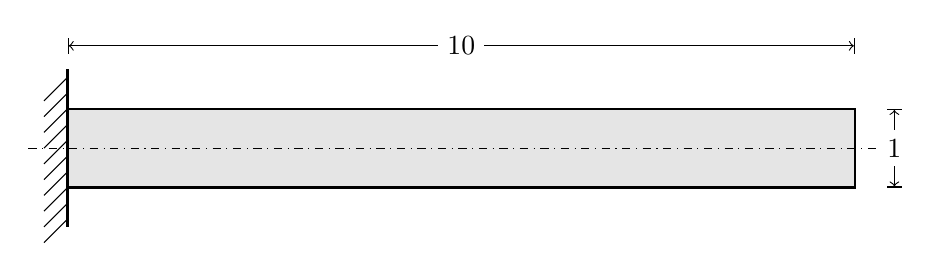
\begin{tikzpicture}
    % Hachuras do engaste (parede à esquerda)
    \foreach \y in {-0.4, -0.2, 0, 0.2, 0.4, 0.6, 0.8, 1.0, 1.2, 1.4} {
        \draw (0, \y) -- (-0.3, \y-0.3);
    }
    % Linha vertical do engaste
    \draw[very thick] (0, -0.5) -- (0, 1.5);

    % Corpo da viga (10x1)
    \filldraw[fill=gray!20, draw=black, thick] (0,0) rectangle (10,1);

    % Linha de centro (eixo neutro)
    \draw[dash dot, thin] (-0.5, 0.5) -- (10.5, 0.5);

    % Cotas de dimensão (opcional, para visualização das proporções)
    \draw[|<->|] (0, 1.8) -- (10, 1.8) node[midway, fill=white] {10};
    \draw[|<->|] (10.5, 0) -- (10.5, 1) node[midway, fill=white] {1};
\end{tikzpicture}